\let\negmedspace\undefined
\let\negthickspace\undefined
\documentclass[journal]{IEEEtran}
\usepackage[a5paper, margin=10mm, onecolumn]{geometry}
\usepackage{lmodern} % Ensure lmodern is loaded for pdflatex
\usepackage{tfrupee} % Include tfrupee package

\setlength{\headheight}{1cm} % Set the height of the header box
\setlength{\headsep}{0mm}     % Set the distance between the header box and the top of the text

\usepackage{gvv-book}
\usepackage{gvv}
\usepackage{cite}
\usepackage{amsmath,amssymb,amsfonts,amsthm}
\usepackage{algorithmic}
\usepackage{graphicx}
\usepackage{textcomp}
\usepackage{xcolor}
\usepackage{txfonts}
\usepackage{listings}
\usepackage{enumitem}
\usepackage{mathtools}
\usepackage{gensymb}
\usepackage{comment}
\usepackage[breaklinks=true]{hyperref}
\usepackage{tkz-euclide} 
\usepackage{listings}
\usepackage{gvv}                                        
\def\inputGnumericTable{}                                 
\usepackage[latin1]{inputenc}                                
\usepackage{color}                                            
\usepackage{array}                                            
\usepackage{longtable}                                       
\usepackage{calc}                                             
\usepackage{multirow}                                         
\usepackage{hhline}                                           
\usepackage{ifthen}                                           
\usepackage{lscape}
\begin{document}

\bibliographystyle{IEEEtran}
\vspace{3cm}

\title{8.3.7}
\author{EE24BTECH11003 - Akshara Sarma Chennubhatla}
% \maketitle
% \newpage
% \bigskip
{\let\newpage\relax\maketitle}
\textbf{Question:}
Find the area enclosed by the parabola $4y = 3x^2$ and the line $2y = 3x + 12$.

\solution\\

The equation of parabola is $g \brak{\vec{x}} = \vec{x}^{\top}\vec{V}\vec{x} + 2 \vec{u}^{\top}\vec{x} + f = 0$. In matrix form, it is given by,
\begin{align}
	\myvec{x & y} \myvec{1 & 0 \\ 0 & 0} \myvec{x \\ y} + 2 \myvec{0 & -\frac{2}{3}} \myvec{x \\ y} + 0 = 0
\end{align}
Line equation is,
\begin{align}
	\vec{x} = \kappa \myvec{2 \\ 3} + \myvec{0 \\ 6}
\end{align}
Intersection of a line and a conic is given by,
\begin{align}
	\kappa_i = \frac{-\vec{m}^{\top}\brak{\vec{Vh}+\vec{u}}\pm\sqrt{\sbrak{\vec{m}^{\top}\brak{\vec{Vh}+\vec{u}}}^2-g\brak{h}\brak{\vec{m}^{\top}\vec{Vm}}}}{\vec{m}^{\top}\vec{Vm}}
\end{align}
For the given conic, $\vec{V}=\myvec{1 & 0 \\ 0 & 0 }, \vec{u} = \myvec{0 \\ -\frac{2}{3}}, f = 0$. For the given line, $\vec{h}=\myvec{0 \\ 6}$, $\vec{m}=\myvec{2 \\ 3}$
\begin{align}	
	\implies \kappa_i = \myvec{-2 \\ 3}, \myvec{4 \\ 12}
\end{align}
The 2 curves meet at the points \myvec{-2\\3} and \myvec{4\\12}. So, the area between the curves is given by,
\begin{align}
	\int{\brak{\frac{3}{2}x + 6} - {\brak{\frac{3}{4}x^2}}}
\end{align}

\textbf{Theoretical Solution:}\\

\begin{align}
	\int{\brak{\frac{3}{2}x + 6} - {\brak{\frac{3}{4}x^2}}}\\
	= \sbrak{\frac{3}{2}\brak{\frac{x^2}{2}} + 6x}_{-2}^{4} - \sbrak{\frac{3}{4}\brak{\frac{x^3}{3}}}_{-2}^{4}\\
	= \brak{24 + 12 - 16} - \brak{2 + 3 - 12}\\
	= 27 sq.units
\end{align}

\textbf{Simulated Solution:}\\

First, we divide the interval $b-a$ into $n$ intervals of equal sizes, each of size $\frac{b-a}{n}$. We shall call each of the $x$ values at the boundaries as $x_1, x_2, x_3,....x_{n+1}$, where $x_1 = a, x_{n+1} = b$ and the step size as $h$. Individual areas are in the shape of a trapezoid. So, we sum the values of the areas of the individual trapezoids to get the value of the definite integral between $a$ and $b$. For the $n_{th}$ trapezoid, the area is given by,
\begin{align}
	A_n = \frac{1}{2} \brak{h} \brak{y\brak{x_n} + y\brak{x_{n+1}}}
\end{align}
Also,
\begin{align}
	A_{n+1} = A_n + \frac{1}{2} h \brak{y_n + y_{n+1}}
\end{align}
Using this equation we can get the total area under the curve by taking the sum of $A_1$ to $A_n$.\\
\begin{align}
	A &= \frac{1}{2} h \brak{y \brak{x_1} + y \brak{x_0}}+ \frac{1}{2} h \brak{y \brak{x_2} + y \brak{x_1}} + \dots + \frac{1}{2} h \brak{y \brak{x_n} + y\brak{x_{n-1}}}\\
	&= h \sbrak{\frac{1}{2} \brak{y \brak{x_0} + y \brak{x_n}} + y \brak{x_1} + \dots + y \brak{x_{n-1}}}
\end{align}
By the first principle of derivatives,\\
\begin{align}
	y\brak{x+h} = y\brak{x} + h y^{\prime}\brak{x}
\end{align}
In this case, to calculate the area enclosed between the line and the parabola, we subtract the $y$ coordinate of the parabola from the $y$ coordinate of the line and then apply the trapezoidal rule on that function.\\
For the parabola,
\begin{align}
	\frac{dy}{dx} = \frac{3x}{2}
\end{align}
For the line,
\begin{align}
	\frac{dy}{dx} = \frac{3}{2}
\end{align}
The general area element in this case is given by,
\begin{align}
	A_n &= \frac{1}{2} h \brak{y\brak{x_n} + \brak{y\brak{x_n} + hy^\prime\brak{x_n}}}\brak{\text{for line}} - \frac{1}{2} h \brak{y\brak{x_n} + \brak{y\brak{x_n} + hy^\prime\brak{x_n}}}\brak{\text{for parabola}}\\
	A_n &= \frac{1}{2} h \brak{3x_n + 12 + h\frac{3}{2} - \frac{3}{2}x_n^2 - h\frac{3x_n}{2}}\\
\end{align}
The general difference equation is given by,
\begin{align}
	A_{n+1} &= A_n + \frac{1}{2}h\brak{3x_n + 12 + h\frac{3}{2} - \frac{3}{2}x_n^2 - h\frac{3x_n}{2}}\\
	x_{n+1} &= x_n + h
\end{align}
By iterating through the required value of $n$, we get the area enclosed between the line and the parabola.\\
Theoretical area $= 27$ sq.units\\
Calculated area through trapezoidal rule $= 26.9815636$ sq.units\\

Below is the plot for line and the parabola
\begin{figure}[h!]
	\centering
	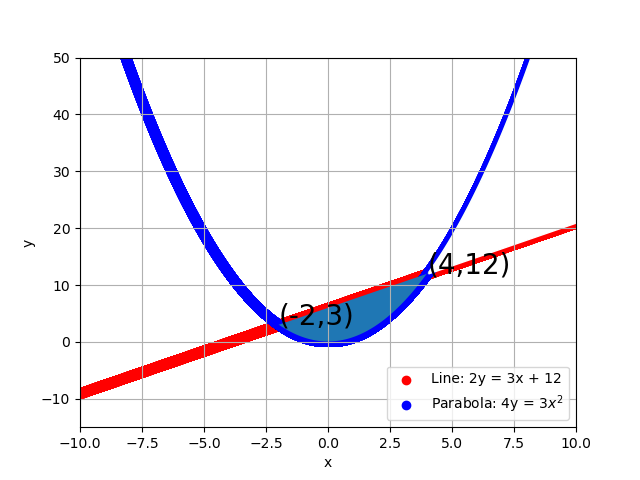
\includegraphics[width=1\columnwidth]{figs/simulated.png}
	\caption{Plot of the line $2y = 3x + 12$ and the parabola = $4y = 3x^2$}
	\label{stemplot}
\end{figure}

\end{document}
